%!TEX root = artem_kotov_v1.tex
\section{Task 4}

\begin{task}
    Определить, какая из величин $a, b, d$ вносит наибольший вклад в уточнение прогноза для величины c (в смысле дисперсии распределения).
\end{task}


Проведенный численный эксперимент показал, что для первой модели условия $\D [c|d] < \D [c|b]$ и $\D [c|d] < \D [c|a]$ выполняются для любых допустимых значений $a \in [75, 90]$, $b \in [500, 600]$ и $d \in [0, 1380]$. Однако для второй модели это оказывается неверным, к сожалению, аналитически показать это строго пока не удалось, т.е. может быть так, что это просто численная ошибка, но я, скорее, склоняюсь к тому, что это свойства модели.

\begin{figure}[H]
    \centering
    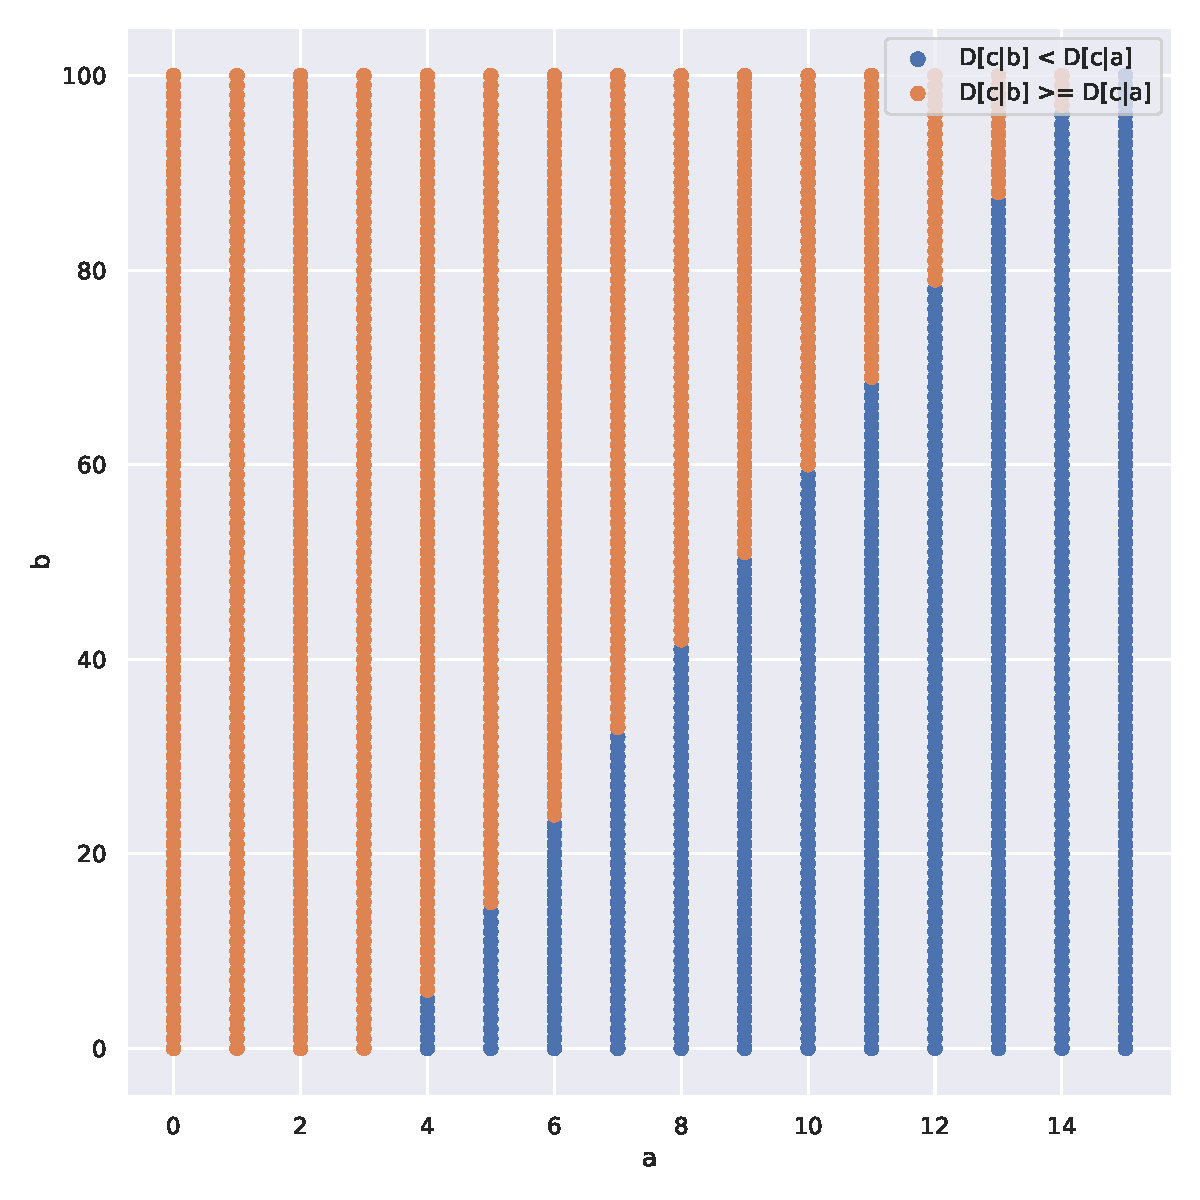
\includegraphics[width=0.7\textwidth]{pics/task4_1.pdf}
    \caption{График множества точек ${(a, b): \D [c|b] < D[c|a]}$ (синий) и ${(a, b): \D [c|b] \ge D[c|a]}$ (оранжевый) для первой модели.}
\end{figure}

\begin{figure}[H]
    \centering
    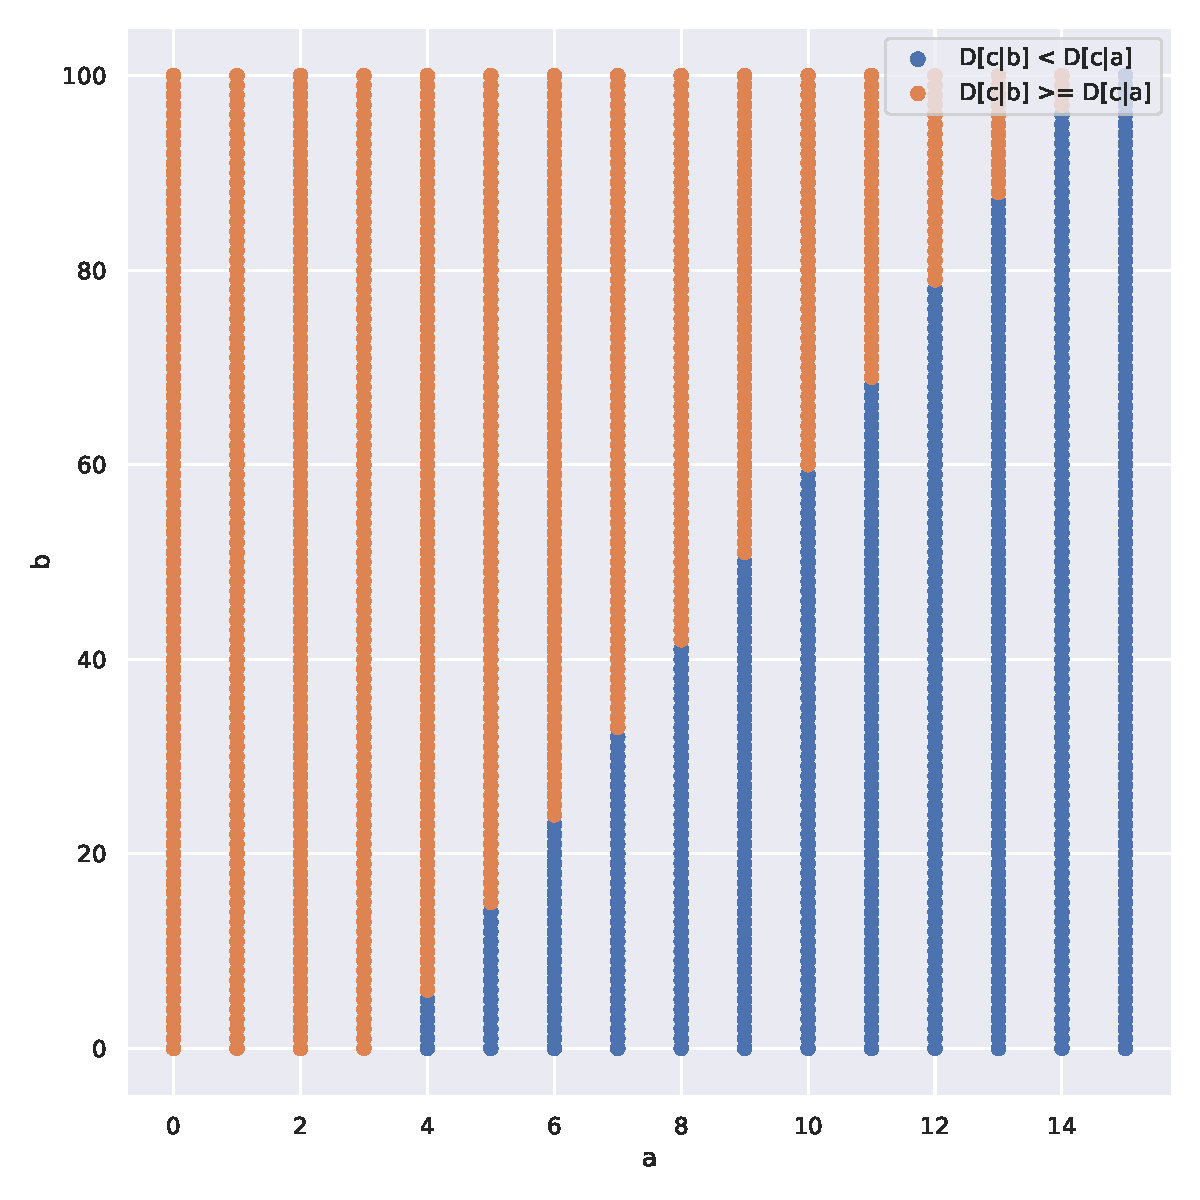
\includegraphics[width=0.7\textwidth]{pics/task4_1.pdf}
    \caption{График множества точек $\{(a, b): \D [c|b] < D[c|a]\}$ (синий) и $\{(a, b): \D [c|b] \ge D[c|a]\}$ (оранжевый) для второй модели.}
\end{figure}

В целом, из графиков можно сделать вывод, что эти множества таки линейно разделимы для обоих моделей.

А теперь попробуем привести показательство: рассмотрим $p(c|ab)$ и заметим, что $a|b = a$, т.к. $a$ и $b$ независимые.

Введем $y = c|b$ и $x = a|b \,\,(=a)$, тогда $c|ab = y|x$
\begin{remark}
    Не важно, в каком порядке обуславливать на $a$ и $b$: сначала $a$, а потом $b$ или наоборот, т.к. $a$ и $b$ независимые.
\end{remark}

По формуле полной вариации:
\begin{gather}
    \D y = \E (\D [y|x]) + \D (\E [y|x]) \\
    \D[y|x] = \D[c|ab] = \D[\Bin(a, p_1) + \Bin(b, p_2)] = a p_1 (1 - p_1) + b p_2 (1 - p_2) \\
    \E_a \D[y|x] = \E a \cdot p_1 (1 - p_1) + \underbrace{b}_{\text{т.к. b не зависит от }a} p_2 (1 - p_2) \\
    \E[y|x] = \E[\Bin(a, p_1) + \Bin(b, p_2)] = a p_1 + b p_2 \\
    \D_a (\E[y|x]) = \D a p_1^2,
\end{gather}
тогда получаем, что
\begin{equation}
    \D[c|b] = \E a \cdot p_1 (1 - p_1) + b p_2 (1 - p_2) + \D a \cdot p_1^2.
\end{equation}
Аналогично
\begin{equation}
    \D[c|a] = \E b \cdot p_2 (1 - p_2) + a p_1 (1 - p_1) + \D b \cdot p_2^2.
\end{equation}

Рассмотрим множество точек, где $\D[c|a] = \D[c|b]$, т.е.
\begin{gather}
    b p_2 (1 - p_2) = C + a p_1 (1 - p_1),
\end{gather}
где $C$ -- некая константа, определяемая через $p_1, p_2, \E b, \E a$.
Заметим, что это уравнение есть уравнение прямой в плоскости $(a, b)$: $b = k a + c$, т.е. множество точек, где $\D[c|a] = \D[c|b]$ есть прямая в плоскости $(a, b)$, т.е. множества действительно линейно разделимы.

Для модели Пуассона все аналогично, разве что для $c|ab$ мы получим $\Poisson(ap_1 + bp_2)$, что в итоге даст:
\begin{gather}
    \D[c|a] = \E a p_1 + bp_2 + \D a p_1 \\
    \D[c|b] = \E b p_2 + ap_1 + \D b p_2,
\end{gather}
что приведет снова к уравнению прямой в плоскости $(a, b)$.
